\documentclass{beamer}

% Theme choice
\usetheme{Madrid} % You can change to e.g., Warsaw, Berlin, CambridgeUS, etc.

% Encoding and font
\usepackage[utf8]{inputenc}
\usepackage[T1]{fontenc}

% Graphics and tables
\usepackage{graphicx}
\usepackage{booktabs}

% Code listings
\usepackage{listings}
\lstset{
basicstyle=\ttfamily\small,
keywordstyle=\color{blue},
commentstyle=\color{gray},
stringstyle=\color{red},
breaklines=true,
frame=single
}

% Math packages
\usepackage{amsmath}
\usepackage{amssymb}

% Colors
\usepackage{xcolor}

% TikZ and PGFPlots
\usepackage{tikz}
\usepackage{pgfplots}
\pgfplotsset{compat=1.18}
\usetikzlibrary{positioning}

% Hyperlinks
\usepackage{hyperref}

% Title information
\title{Week 5: Data Structures}
\author{Your Name}
\institute{Your Institution}
\date{\today}

\begin{document}

\frame{\titlepage}

\begin{frame}[fragile]
    \frametitle{Very Rough Rules About Data Structures}
    \begin{itemize}
        \item Arrays are almost always the best choice for both speed and memory, so other structures are mostly special cases.
        \item Stacks and queues are interchangeable because they both store items in a list.
        \item Performance analysis is less important than using the structure students already remember from syntax practice.
    \end{itemize}
\end{frame}

\begin{frame}[fragile]
    \frametitle{Introduction to Data Structures}
    \begin{block}{Overview}
        Data structures are specialized formats for organizing, processing, and storing data. 
        They are essential for managing large amounts of information efficiently.
    \end{block}
\end{frame}

\begin{frame}[fragile]
    \frametitle{Importance of Data Structures}
    \begin{enumerate}
        \item \textbf{Efficiency:} 
            Data structures enable optimized storage and retrieval of data.
            For example, a hash table can reduce lookup time from \(O(n)\) to \(O(1)\).
        \item \textbf{Organization:} 
            Proper data structure choices logically categorize data, aiding understanding.
        \item \textbf{Performance:} 
            They significantly enhance algorithm performance.
        \item \textbf{Scalability:} 
            Well-designed structures allow applications to scale without performance loss.
    \end{enumerate}
\end{frame}

\begin{frame}[fragile]
    \frametitle{Real-World Examples}
    \begin{itemize}
        \item \textbf{Arrays:} Fast access by index (e.g., storing student grades).
        \item \textbf{Linked Lists:} Handle dynamic data with frequent insertions/deletions (e.g., music playlists).
        \item \textbf{Stacks and Queues:} Manage tasks, such as Undo actions and print jobs.
        \item \textbf{Graphs:} Represent networks, including social media connections.
    \end{itemize}
\end{frame}

\begin{frame}[fragile]
    \frametitle{Choosing a Data Structure}
    \begin{block}{Scenario: Managing User Accounts}
        Considerations for choosing a data structure:
        \begin{itemize}
            \item \textbf{Frequent Access:} Use a hash table for quick lookups.
            \item \textbf{Sorted Data:} Consider a binary search tree.
            \item \textbf{Frequent Insertions/Deletions:} A linked list may be ideal.
        \end{itemize}
    \end{block}
\end{frame}

\begin{frame}[fragile]
    \frametitle{Key Takeaways}
    \begin{itemize}
        \item Choosing the right data structure impacts software design.
        \item Understanding data structures is foundational for mastering algorithms.
        \item Data structures have critical roles in databases, game development, and networking.
    \end{itemize}
\end{frame}

\begin{frame}[fragile]
    \frametitle{What are Data Structures? - Definition}
    Data structures are specialized formats for organizing, processing, and storing data in a computer. 
    They enable efficient data management and provide a way to handle large amounts of data seamlessly.
\end{frame}

\begin{frame}[fragile]
    \frametitle{What are Data Structures? - Purpose}
    \begin{itemize}
        \item \textbf{Efficient Data Management:} Allows for quick access and modification of data.
        \item \textbf{Optimized Resource Usage:} Minimizes memory usage and reduces time complexity in data operations.
        \item \textbf{Problem Solving:} Serves as foundational building blocks for algorithms and aids in solving complex computational problems.
    \end{itemize}
\end{frame}

\begin{frame}[fragile]
    \frametitle{What are Data Structures? - Functionality & Example}
    \begin{itemize}
        \item \textbf{Data Storage:} Mechanisms to store data according to operations (searching, sorting, iterating).
        \item \textbf{Data Retrieval:} Different structures enable various speeds and methods for accessing data.
        \item \textbf{Data Manipulation:} Supports operations like adding, updating, or removing data efficiently.
    \end{itemize}

    \vspace{10pt}
    
    \textbf{Example: Shopping Cart in E-commerce Application}
    \begin{block}{Illustration}
        \texttt{Shopping Cart:} \\
        \texttt{- Items: [Item1, Item2, Item3]} \\
        \texttt{- Attributes:} \{ \\
        \texttt{   Item1: \{ price: \$10, quantity: 2 \},} \\
        \texttt{   Item2: \{ price: \$15, quantity: 1 \},} \\
        \texttt{   Item3: \{ price: \$8, quantity: 3 \} \\ 
        \texttt{ \}}
    \end{block}
\end{frame}

\begin{frame}[fragile]
    \frametitle{What are Data Structures? - Key Points}
    \begin{itemize}
        \item Data structures are essential for creating efficient algorithms.
        \item Different types of data structures serve different purposes - no one-size-fits-all.
        \item Choosing the right data structure can drastically affect performance in terms of speed and memory use.
    \end{itemize}

    \vspace{10pt}

    By understanding and utilizing various data structures, software engineers can write efficient, maintainable, and scalable code that can handle diverse data requirements effectively.

    \vspace{10pt}
    
    \textbf{Transition:} Next, we’ll dive into specific types of data structures, examining their unique characteristics and applications.
\end{frame}

\begin{frame}[fragile]
    \frametitle{Common Types of Data Structures - Introduction}
    \begin{block}{Introduction to Data Structures}
        Data structures are essential components in computer science that organize and store data in a way that enables efficient access and modification. Different types of data structures cater to various needs and tasks in programming, enabling developers to utilize memory and processing power effectively.
    \end{block}
\end{frame}

\begin{frame}[fragile]
    \frametitle{Common Types of Data Structures - Arrays}
    \begin{itemize}
        \item \textbf{Definition}: An array is a collection of elements identified by index or key, holding a fixed-size sequential collection of elements of the same type.
        \item \textbf{Characteristics}: 
        \begin{itemize}
            \item Fixed size once declared
            \item Elements are stored in contiguous memory locations
            \item Supports efficient random access using an index
        \end{itemize}
        \item \textbf{Example}: 
        \begin{lstlisting}
int[] numbers = {1, 2, 3, 4, 5};  // C# code
        \end{lstlisting}
    \end{itemize}
\end{frame}

\begin{frame}[fragile]
    \frametitle{Common Types of Data Structures - Lists and Trees}
    \begin{enumerate}
        \item \textbf{Lists}
        \begin{itemize}
            \item \textbf{Definition}: A list is a collection that can grow or shrink in size, allowing for dynamic modification of data. 
            \item \textbf{Characteristics}: 
            \begin{itemize}
                \item Dynamic size, can add or remove elements
                \item Often implemented using nodes (in linked lists)
                \item Allows for traversal, insertion, and deletion of elements
            \end{itemize}
            \item \textbf{Example}: 
            \begin{lstlisting}
List<int> numbers = new List<int>();  // C# code
numbers.Add(1);   // Add elements
numbers.Remove(1); // Remove elements
            \end{lstlisting}
        \end{itemize}

        \item \textbf{Trees}
        \begin{itemize}
            \item \textbf{Definition}: A tree is a hierarchical data structure characterized by nodes linked by edges.
            \item \textbf{Characteristics}: 
            \begin{itemize}
                \item Non-linear structure, branches out from a single root
                \item Each node can have multiple children
                \item Used to represent hierarchical data such as file systems
            \end{itemize}
            \item \textbf{Example:}
            \begin{verbatim}
            Comprising of nodes:
                 A               
                / \
               B   C         
              / \   \
             D   E   F
            \end{verbatim}
        \end{itemize}
    \end{enumerate}
\end{frame}

\begin{frame}[fragile]
    \frametitle{Arrays - Definition}
    \begin{block}{Definition}
        An \textbf{array} is a collection of items stored at contiguous memory locations. 
        It is a fundamental data structure used to store multiple values of the same type in a single variable.
    \end{block}
\end{frame}

\begin{frame}[fragile]
    \frametitle{Arrays - Properties}
    \begin{enumerate}
        \item \textbf{Fixed Size}: The size of an array must be defined at the time of its creation and cannot be changed later.
        \item \textbf{Homogeneous Elements}: All elements in an array are of the same data type (e.g., integers, characters).
        \item \textbf{Index-Based Access}: Each element can be accessed directly using an index, starting typically at 0.
        \item \textbf{Continuous Memory Allocation}: Arrays are stored in contiguous memory locations, allowing for quick access.
    \end{enumerate}
\end{frame}

\begin{frame}[fragile]
    \frametitle{Arrays - Code Examples}
    \begin{block}{Example of Array Declaration}
        In different programming languages, arrays can be declared as follows:
        \begin{lstlisting}[language=Python]
my_array = [10, 20, 30, 40, 50]  # Array of integers
        \end{lstlisting}
        \begin{lstlisting}[language=Java]
int[] myArray = {10, 20, 30, 40, 50};  // Array of integers
        \end{lstlisting}
        \begin{lstlisting}[language=C++]
int myArray[5] = {10, 20, 30, 40, 50};  // Array of integers
        \end{lstlisting}
    \end{block}
    
    \begin{block}{Iterating Over an Array}
        Here’s how to iterate through an array to print its elements:
        \begin{lstlisting}[language=Python]
my_array = [10, 20, 30, 40, 50]
for element in my_array:
    print(element)  # Output: 10 20 30 40 50
        \end{lstlisting}
    \end{block}
\end{frame}

\begin{frame}[fragile]
    \frametitle{Lists - Overview}
    \begin{block}{Understanding Lists in Data Structures}
        A list is a linear data structure that allows the storage of a sequence of elements, where each element can be of any type, including objects.
    \end{block}
    
    \begin{block}{Summary}
        - Lists can dynamically grow or shrink.
        - They can be singly-linked or doubly-linked.
        - Each type offers unique advantages and disadvantages.
    \end{block}
\end{frame}

\begin{frame}[fragile]
    \frametitle{Singly-Linked List}
    \begin{itemize}
        \item \textbf{Structure:}
        \begin{itemize}
            \item Each node contains two components: the data and a pointer to the next node.
            \item The first node is the head, and the last node points to NULL.
        \end{itemize}
        
        \item \textbf{Advantages:}
        \begin{itemize}
            \item Dynamic Size: Can grow and shrink in size as needed.
            \item Efficient Removals: Easy to add/remove nodes without reallocation.
        \end{itemize}
        
        \item \textbf{Disadvantages:}
        \begin{itemize}
            \item Sequential Access: Must start from the head to traverse.
            \item Extra Memory: Uses extra memory for storing pointers.
        \end{itemize}
        
        \item \textbf{Example Representation:}
        \begin{center}
            Head $\rightarrow$ Node1 (data) $\rightarrow$ Node2 (data) $\rightarrow$ NULL
        \end{center}
    \end{itemize}
\end{frame}

\begin{frame}[fragile]
    \frametitle{Singly-Linked List - Key Operation}
    \begin{block}{Key Operation: Insertion at Head}
        \begin{lstlisting}[language=Python]
def insert_head(head, new_data):
    new_node = Node(new_data)
    new_node.next = head
    return new_node
        \end{lstlisting}
    \end{block}
\end{frame}

\begin{frame}[fragile]
    \frametitle{Doubly-Linked List}
    \begin{itemize}
        \item \textbf{Structure:}
        \begin{itemize}
            \item Each node has three components: a pointer to the previous node, the data, and a pointer to the next node.
            \item Both forward and backward traversal is possible.
        \end{itemize}
        
        \item \textbf{Advantages:}
        \begin{itemize}
            \item Bidirectional Traversal: Can traverse in both directions.
            \item Easier Deletion: Can access the previous node for easy deletions.
        \end{itemize}
        
        \item \textbf{Disadvantages:}
        \begin{itemize}
            \item More Memory: Requires more storage for additional pointers.
            \item More Complex: Insertion and deletion operations are more complex.
        \end{itemize}
        
        \item \textbf{Example Representation:}
        \begin{center}
            NULL $\leftarrow$ Node1 (data) $\leftrightarrow$ Node2 (data) $\leftrightarrow$ Node3 (data) $\rightarrow$ NULL
        \end{center}
    \end{itemize}
\end{frame}

\begin{frame}[fragile]
    \frametitle{Doubly-Linked List - Key Operation}
    \begin{block}{Key Operation: Insertion at Tail}
        \begin{lstlisting}[language=Python]
def insert_tail(tail, new_data):
    new_node = Node(new_data)
    tail.next = new_node
    new_node.prev = tail
    return new_node
        \end{lstlisting}
    \end{block}
\end{frame}

\begin{frame}[fragile]
    \frametitle{Summary and Applications of Lists}
    \begin{itemize}
        \item \textbf{Summary:}
        \begin{itemize}
            \item Singly-Linked Lists are efficient for memory usage and simple forward operations.
            \item Doubly-Linked Lists provide flexibility for backward traversals but have higher memory overhead.
        \end{itemize}
        
        \item \textbf{Applications of Lists:}
        \begin{itemize}
            \item Implementation of stacks and queues.
            \item Adjacency lists for graph representation.
            \item Dynamic arrays where capacity can fluctuate.
        \end{itemize}
    \end{itemize}
\end{frame}

\begin{frame}[fragile]
    \frametitle{Trees - Definition}
    \begin{block}{Understanding Tree Data Structures}
        A tree is a hierarchical data structure that consists of nodes connected by edges. 
        Each tree has a single root node with zero or more child nodes, and the connections 
        between nodes are referred to as edges.
    \end{block}
    
    \begin{itemize}
        \item \textbf{Node:} A fundamental part of a tree, which contains data.
        \item \textbf{Root:} The top node in a tree.
        \item \textbf{Leaf:} A node with no children.
        \item \textbf{Height:} The length of the longest path from the root to a leaf.
        \item \textbf{Subtree:} A tree that consists of a node and all its descendants.
    \end{itemize}
\end{frame}

\begin{frame}[fragile]
    \frametitle{Trees - Types of Trees}
    \begin{block}{Types of Trees}
        \begin{itemize}
            \item \textbf{Binary Trees:}
            \begin{itemize}
                \item A tree structure where each node has at most two children, referred to as the left and right child.
            \end{itemize}
            \begin{center}
            \texttt{
            \begin{tabular}{c}
                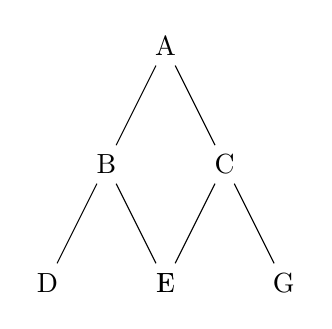
\begin{tikzpicture}
                    \node {A}
                    child {node {B}
                           child {node {D}}
                           child {node {E}}
                    }
                    child {node {C}
                           child {node {F}}
                           child {node {G}}
                    };
                \end{tikzpicture}
            \end{tabular}}
            \end{center}
            \item \textbf{Binary Search Trees (BST):}
            \begin{itemize}
                \item A special type of binary tree where the left child of a node contains 
                only nodes with keys less than the node’s key, and the right child only contains 
                nodes with keys greater than the node’s key.
            \end{itemize}
            \begin{center}
            \texttt{
            \begin{tabular}{c}
                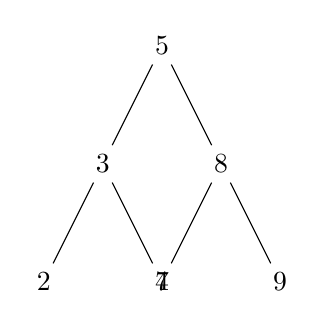
\begin{tikzpicture}
                    \node {5}
                    child {node {3}
                           child {node {2}}
                           child {node {4}}
                    }
                    child {node {8}
                           child {node {7}}
                           child {node {9}}
                    };
                \end{tikzpicture}
            \end{tabular}}
            \end{center}
        \end{itemize}
    \end{block}
\end{frame}

\begin{frame}[fragile]
    \frametitle{Trees - Applications and Key Points}
    \begin{block}{Applications of Trees}
        \begin{itemize}
            \item \textbf{Data Management:} File systems use trees for organizing files and directories.
            \item \textbf{Databases:} B-trees and Red-Black trees help with efficient data access and indexing.
            \item \textbf{Network Routing:} Trees can model the structure of networks for routing algorithms.
            \item \textbf{Expression Parsing:} Abstract Syntax Trees (ASTs) represent the structure of expressions and statements in compilers.
        \end{itemize}
    \end{block}
    
    \begin{block}{Key Points}
        \begin{itemize}
            \item The tree structure is fundamental for efficient searching and sorting techniques.
            \item Different types of trees (e.g., binary, binary search) serve distinct purposes and optimize different operations.
        \end{itemize}
    \end{block}
\end{frame}

\begin{frame}[fragile]
    \frametitle{Trees - Basic Operations on a Binary Search Tree (BST)}
    \begin{block}{Basic Operations}
        \begin{enumerate}
            \item \textbf{Insertion:} Place a new node in the correct position to maintain the BST properties.
            \item \textbf{Searching:} Start from the root; traverse left if the target is smaller, and right if larger until found.
            \item \textbf{Traversal Techniques:}
            \begin{itemize}
                \item \textbf{In-order traversal:} Left, Root, Right (produces sorted order).
                \item \textbf{Pre-order traversal:} Root, Left, Right.
                \item \textbf{Post-order traversal:} Left, Right, Root.
            \end{itemize}
        \end{enumerate}
    \end{block}

    \begin{lstlisting}[language=Python]
# Python Code Snippet for Inserting in a BST
class Node:
    def __init__(self, key):
        self.left = None
        self.right = None
        self.val = key

def insert(root, key):
    if root is None:
        return Node(key)
    else:
        if key < root.val:
            root.left = insert(root.left, key)
        else:
            root.right = insert(root.right, key)
    return root
    \end{lstlisting}
\end{frame}

\begin{frame}[fragile]
    \frametitle{Why Choose One Data Structure Over Another? - Part 1}
    \begin{block}{Introduction}
        Data structures are fundamental components of programming that organize and store data efficiently. Selecting the appropriate data structure for a specific problem is crucial, as it can significantly affect performance, ease of implementation, and the overall effectiveness of a program.
    \end{block}
\end{frame}

\begin{frame}[fragile]
    \frametitle{Factors Influencing Choice of Data Structure - Part 2}
    \begin{enumerate}
        \item \textbf{Efficiency}
            \begin{itemize}
                \item \textbf{Time Complexity:} The speed at which operations (insert, delete, search) can be performed.
                \begin{itemize}
                    \item Example: Inserting into a linked list (O(1) for head insertion) vs. searching in an unsorted array (O(n)).
                \end{itemize}
                \item \textbf{Space Complexity:} The amount of memory required by a data structure.
                \begin{itemize}
                    \item Example: A hash table may require more space than an array but offers faster look-ups.
                \end{itemize}
            \end{itemize}
        \item \textbf{Ease of Implementation}
            \begin{itemize}
                \item Some data structures require significant coding effort to implement correctly.
                \begin{itemize}
                    \item Example: Implementing a queue using an array is simpler than using a double-ended linked list.
                \end{itemize}
            \end{itemize}
    \end{enumerate}
\end{frame}

\begin{frame}[fragile]
    \frametitle{Use Cases and Scalability - Part 3}
    \begin{enumerate}
        \setcounter{enumi}{2}
        \item \textbf{Use Case}
            \begin{itemize}
                \item Understanding specific application requirements is key to selecting the right data structure.
                \begin{itemize}
                    \item Example Scenarios:
                    \begin{itemize}
                        \item \textbf{Stacks:} Backtracking algorithms (e.g., navigating browser history).
                        \item \textbf{Queues:} Scheduling tasks (e.g., print job management).
                        \item \textbf{Graphs:} Representing networks (e.g., social connections).
                    \end{itemize}
                \end{itemize}
            \end{itemize}
        \item \textbf{Scalability}
            \begin{itemize}
                \item Performance as dataset size grows is crucial. 
                \begin{itemize}
                    \item Example: A balanced binary search tree (like an AVL tree) maintains O(log n) search time efficiently as it grows.
                \end{itemize}
            \end{itemize}
    \end{enumerate}
\end{frame}

\begin{frame}[fragile]
    \frametitle{Summary and Example Code - Part 4}
    \begin{block}{Summary}
        \begin{itemize}
            \item Choosing the right data structure involves evaluating factors such as efficiency, implementation complexity, use case alignment, and scalability.
            \item Understanding these factors helps developers write optimal and maintainable code.
        \end{itemize}
    \end{block}
    \begin{block}{Example Code Snippet}
        \begin{lstlisting}[language=Python]
class Stack:
    def __init__(self):
        self.items = []

    def push(self, item):
        self.items.append(item)

    def pop(self):
        if not self.is_empty():
            return self.items.pop()
        raise Exception("Stack is empty")
    
    def is_empty(self):
        return len(self.items) == 0
        \end{lstlisting}
    \end{block}
\end{frame}

\begin{frame}[fragile]
    \frametitle{Use Cases and Applications}
    In software development, the choice of data structure is crucial as it directly impacts the efficiency, performance, and scalability of applications. Below we explore some common data structures along with real-world scenarios where they are effectively utilized.
\end{frame}

\begin{frame}[fragile]
    \frametitle{1. Arrays}
    \begin{itemize}
        \item \textbf{Description:} A collection of elements identified by index or key.
        \item \textbf{Use Case:} Storing a fixed-size list of items, like a list of student names or the days of the week.
        \item \textbf{Example:}
        \begin{lstlisting}[language=Python]
days_of_week = ["Monday", "Tuesday", "Wednesday", "Thursday", "Friday", "Saturday", "Sunday"]
        \end{lstlisting}
        \item \textbf{Key Point:} Efficient for accessing elements by an index.
    \end{itemize}
\end{frame}

\begin{frame}[fragile]
    \frametitle{2. Linked Lists}
    \begin{itemize}
        \item \textbf{Description:} A linear collection of data elements, where each element points to the next.
        \item \textbf{Use Case:} Implementing dynamic data structures such as a playlist in a music player.
        \item \textbf{Example:}
        \begin{lstlisting}[language=Python]
class Node:
    def __init__(self, data):
        self.data = data
        self.next = None

# Creating linked list nodes
song1 = Node("Song A")
song2 = Node("Song B")
song1.next = song2  # Linking songs
        \end{lstlisting}
        \item \textbf{Key Point:} Offers efficient insertions/deletions.
    \end{itemize}
\end{frame}

\begin{frame}[fragile]
    \frametitle{3. Stacks}
    \begin{itemize}
        \item \textbf{Description:} A collection of elements that follows the Last In First Out (LIFO) principle.
        \item \textbf{Use Case:} Undo mechanisms in text editors, where the last action must be undone first.
        \item \textbf{Example:}
        \begin{lstlisting}[language=Python]
stack = []
stack.append("Action 1")
stack.append("Action 2")
last_action = stack.pop()  # Removes "Action 2"
        \end{lstlisting}
        \item \textbf{Key Point:} Great for management of recursive function calls.
    \end{itemize}
\end{frame}

\begin{frame}[fragile]
    \frametitle{4. Queues}
    \begin{itemize}
        \item \textbf{Description:} A collection of elements that follows the First In First Out (FIFO) principle.
        \item \textbf{Use Case:} Managing requests in a print queue where documents are printed in order.
        \item \textbf{Example:}
        \begin{lstlisting}[language=Python]
from collections import deque

queue = deque()
queue.append("Document 1")
queue.append("Document 2")
next_document = queue.popleft()  # Removes "Document 1"
        \end{lstlisting}
        \item \textbf{Key Point:} Ideal for scheduling and order maintenance tasks.
    \end{itemize}
\end{frame}

\begin{frame}[fragile]
    \frametitle{5. Hash Tables}
    \begin{itemize}
        \item \textbf{Description:} A structure that implements an associative array, allowing for fast data retrieval based on keys.
        \item \textbf{Use Case:} Storing user data where usernames (keys) are mapped to user IDs (values).
        \item \textbf{Example:}
        \begin{lstlisting}[language=Python]
user_data = {
    "user1": 101,
    "user2": 102,
    "user3": 103
}
user_id = user_data["user1"]  # Fetching user ID for 'user1'
        \end{lstlisting}
        \item \textbf{Key Point:} Provides average O(1) time complexity for searches.
    \end{itemize}
\end{frame}

\begin{frame}[fragile]
    \frametitle{6. Trees (Binary Trees and Binary Search Trees)}
    \begin{itemize}
        \item \textbf{Description:} A hierarchical structure with a root node and sub-nodes that form a parent-child relationship.
        \item \textbf{Use Case:} Implementing a file system directory structure where folders can contain files and subfolders.
        \item \textbf{Example:}
        \begin{lstlisting}[language=Python]
class TreeNode:
    def __init__(self, value):
        self.value = value
        self.left = None
        self.right = None
        \end{lstlisting}
        \item \textbf{Key Point:} Enables efficient searching, insertion, and deletion operations.
    \end{itemize}
\end{frame}

\begin{frame}
    \frametitle{Conclusion}
    \begin{itemize}
        \item Choosing the right data structure can enhance performance and scalability.
        \item Understanding use cases — from managing playlists with linked lists to print queues — is essential.
        \item Prepare for interactive coding exercises in the next slide.
    \end{itemize}
    \textbf{Remember:} Always consider efficiency and specific application needs when selecting a data structure.
\end{frame}

\begin{frame}[fragile]
    \frametitle{Hands-On Coding Exercises - Overview}
    In this section, we will engage in hands-on coding exercises that allow us to implement and manipulate several common data structures. This interactive approach will solidify our understanding of how these structures work and their practical applications.
\end{frame}

\begin{frame}
    \frametitle{Key Data Structures to Explore}
    \begin{itemize}
        \item \textbf{Arrays}
        \item \textbf{Linked Lists}
        \item \textbf{Stacks}
        \item \textbf{Queues}
        \item \textbf{Dictionaries/Hash Maps}
        \item \textbf{Trees}
        \item \textbf{Graphs}
    \end{itemize}
\end{frame}

\begin{frame}
    \frametitle{Objectives}
    \begin{enumerate}
        \item \textbf{Understand} the behavior and properties of various data structures.
        \item \textbf{Implement} basic operations such as insertion, deletion, and traversal.
        \item \textbf{Manipulate} data to see the effects in real-time.
    \end{enumerate}
\end{frame}

\begin{frame}[fragile]
    \frametitle{Hands-On Coding Exercises - Array Example}
    \textbf{Task:} Write a function that rotates an array to the right by k steps.

    \begin{lstlisting}[language=Python]
def rotate_array(arr, k):
    n = len(arr)
    k = k % n
    return arr[-k:] + arr[:-k]

# Example Usage:
print(rotate_array([1, 2, 3, 4, 5], 2))  # Output: [4, 5, 1, 2, 3]
    \end{lstlisting}
\end{frame}

\begin{frame}[fragile]
    \frametitle{Hands-On Coding Exercises - Linked List Example}
    \textbf{Task:} Implement a method to reverse a linked list.

    \begin{lstlisting}[language=Python]
class Node:
    def __init__(self, data):
        self.data = data
        self.next = None

def reverse_linked_list(head):
    previous = None
    current = head
    while current:
        next_node = current.next
        current.next = previous
        previous = current
        current = next_node
    return previous
    \end{lstlisting}
\end{frame}

\begin{frame}[fragile]
    \frametitle{Hands-On Coding Exercises - Stack Example}
    \textbf{Task:} Create a stack using a list and implement push/pop operations.

    \begin{lstlisting}[language=Python]
stack = []
def push(value):
    stack.append(value)

def pop():
    return stack.pop() if stack else None
    \end{lstlisting}
\end{frame}

\begin{frame}[fragile]
    \frametitle{Hands-On Coding Exercises - Queue Example}
    \textbf{Task:} Implement a queue using collections.deque.

    \begin{lstlisting}[language=Python]
from collections import deque
queue = deque()

def enqueue(value):
    queue.append(value)

def dequeue():
    return queue.popleft() if queue else None
    \end{lstlisting}
\end{frame}

\begin{frame}[fragile]
    \frametitle{Hands-On Coding Exercises - Dictionary Example}
    \textbf{Task:} Count the frequency of elements in a list.

    \begin{lstlisting}[language=Python]
def count_frequencies(nums):
    frequency = {}
    for num in nums:
        frequency[num] = frequency.get(num, 0) + 1
    return frequency
    \end{lstlisting}
\end{frame}

\begin{frame}[fragile]
    \frametitle{Hands-On Coding Exercises - Tree Example}
    \textbf{Task:} Perform a level-order traversal of a binary tree.

    \begin{lstlisting}[language=Python]
from collections import deque
class TreeNode:
    def __init__(self, value):
        self.value = value
        self.left = None
        self.right = None

def level_order_traversal(root):
    if not root:
        return []
    result, queue = [], deque([root])
    while queue:
        node = queue.popleft()
        result.append(node.value)
        if node.left: queue.append(node.left)
        if node.right: queue.append(node.right)
    return result
    \end{lstlisting}
\end{frame}

\begin{frame}
    \frametitle{Key Takeaways}
    \begin{itemize}
        \item Hands-on coding practice is vital for mastering data structure concepts.
        \item Regular interaction with coding problems enhances problem-solving skills.
        \item Each data structure serves different scenarios and performance needs.
    \end{itemize}
\end{frame}

\begin{frame}[fragile]
    \frametitle{Conclusion and Key Takeaways - Overview}
    As we wrap up our week on Data Structures, it is vital to consolidate our understanding of the key concepts explored. The choice of data structures plays a crucial role in software engineering and can significantly impact algorithm efficiency, memory usage, and overall application performance.
\end{frame}

\begin{frame}[fragile]
    \frametitle{Key Points Covered}
    \begin{enumerate}
        \item \textbf{Understanding Data Structures:}
        \begin{itemize}
            \item A specialized format for organizing and managing data.
            \item Common types:
            \begin{itemize}
                \item Arrays: Fixed-size, sequential collections.
                \item Linked Lists: Dynamic collections of nodes.
                \item Stacks: Last-In-First-Out (LIFO) structures.
                \item Queues: First-In-First-Out (FIFO) structures.
                \item Trees: Hierarchical structures with nodes.
                \item Graphs: Structures representing networks.
            \end{itemize}
        \end{itemize}
        
        \item \textbf{Choosing the Right Data Structure:}
        \begin{itemize}
            \item Depends on problem requirements.
            \item Speed of access, dynamic resizing, and insertion/deletion efficiency are key factors.
        \end{itemize}
    \end{enumerate}
\end{frame}

\begin{frame}[fragile]
    \frametitle{Efficiency Considerations}
    \begin{itemize}
        \item \textbf{Time Complexity:} 
        \begin{itemize}
            \item Insertion in a linked list is O(1), while for arrays, it is O(n).
        \end{itemize}
        
        \item \textbf{Space Complexity:} 
        \begin{itemize}
            \item Some structures, like trees, may require additional memory for pointers.
        \end{itemize}
    \end{itemize}
\end{frame}

\begin{frame}[fragile]
    \frametitle{Examples of Data Structures in Action}
    \begin{itemize}
        \item \textbf{Web Browser's Back Button:}
        \begin{itemize}
            \item \textit{Ideal Data Structure:} Stack for easy backtracking of pages.
        \end{itemize}
        
        \item \textbf{Managing Tasks:}
        \begin{itemize}
            \item \textit{Ideal Data Structure:} Queue for processing tasks in order of arrival.
        \end{itemize}
    \end{itemize}
\end{frame}

\begin{frame}[fragile]
    \frametitle{Emphasis on Importance}
    \begin{itemize}
        \item \textbf{Performance Optimization:}
        Choosing the right data structure can lead to significant performance gains. 
        \item \textbf{Example:} Utilizing a Binary Search Tree can achieve O(log n) complexity compared to O(n^2) for Bubble Sort.
        
        \item \textbf{Real-World Applications:}
        \begin{itemize}
            \item Underlie many systems from databases to search engines, enhancing software designs.
        \end{itemize}
    \end{itemize}
\end{frame}

\begin{frame}[fragile]
    \frametitle{Conclusion}
    In software engineering, the correct data structure is foundational to creating efficient algorithms and scalable applications. Always consider the nature of your data and application requirements to improve coding practices and enhance user experience.
    
    \vspace{0.5cm}
    \textit{Consider this conclusion not just an ending, but a stepping stone to further explore advanced data structures!}
\end{frame}


\end{document}
